
\documentclass{beamer}

\usepackage{graphicx}
\usepackage{amsmath}
\usepackage{amssymb}
\usepackage{subfiles}
\begin{document}

		%=========================================================== %
		\begin{frame}
			\begin{figure}
				\centering
				
\includegraphics[width=0.6\linewidth]{rlogo}
			\end{figure}
			\LARGE
			\[ \mbox{The \texttt{R} Community} \] \bigskip
			
		\end{frame}
	%============================================================ %
	\begin{frame}
	
	\frametitle{R groups in UK and Ireland}
		\textbf{User Groups}
		\Large
		\begin{itemize}
			
			\item Useful: Meetup.com and Twitter
			
			\item Dublin \texttt{R}, LondonR, Sheffield R, EdinbR
			
			\item Twitter: \texttt{\#}\texttt{rstats} and \texttt{\#}\texttt{rstats}
			
			\item What happens? Beer and Pizza?
			
		\end{itemize}
		
	\end{frame}
\begin{frame}
\begin{figure}
	\centering
	
\includegraphics[width=0.9\linewidth]{dublinrlogo.jpg}
\end{figure}
\LARGE
\[ \mbox{Dublin \texttt{R} Community} \] \bigskip
\end{frame}	
%==================================================================== %
\begin{frame}
	\begin{figure}
		\centering
		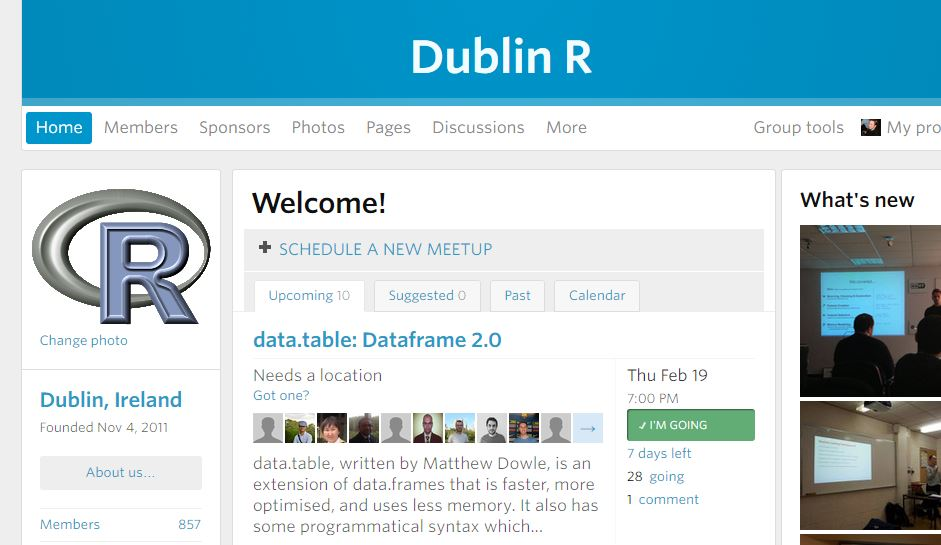
\includegraphics[width=0.99\linewidth]{dublinrpage.jpg}
	\end{figure}
	
\end{frame}	


\begin{frame}
	\begin{figure}
		\centering
		
\includegraphics[width=0.99\linewidth]{revoR.jpg}
	\end{figure}
	
\end{frame}	

%===================================================================== %
\begin{frame}
	
\begin{figure}
\centering

\includegraphics[width=0.85\linewidth]{LondonRlogo}\\

\includegraphics[width=0.55\linewidth]{mangosolutions}
\end{figure}


\Large
\[ \mbox{www.LondonR.org} \]

\end{frame}

%================================================================= %
\begin{frame}

\frametitle{\texttt{R} users groups in UK and Ireland}
\large
	\textbf{User Group Formats}
	\begin{itemize}

	\item \textbf{Dublin R} - Monthly meeting  - 1 hour talk. \\ Also a monthly 2-hour workshop
	\item  \textit{(Workshops on hold due to lack of suitable venues)}
		\item \textbf{LondonR} - Quarterly meetings 100-200 people in attendance. \\ Three or four 20 minutes talks.
		\item \textit{(also 2-3 hour free workshop in same venue beforehand)}	
	\item Other Groups: Sheffield R, Manchester R, Cardiff R and EdinbR - were very recently started
	\end{itemize}
\end{frame}
%================================================================== %

\begin{frame}
\begin{figure}
\centering

\includegraphics[width=1.11\linewidth]{meetuplogo}
\end{figure}
\end{frame}
\begin{frame}
	\begin{figure}
		\centering
		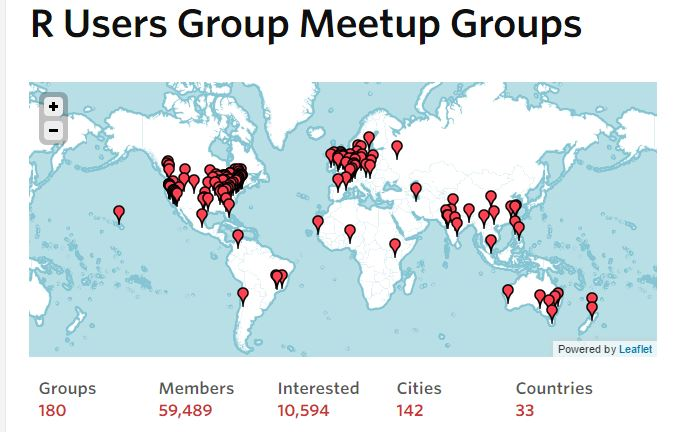
\includegraphics[width=1.11\linewidth]{rusergroupmap}
	\end{figure}
\end{frame}
%================================================================== %
\begin{frame}
	
\frametitle{Interaction with Other Entities}
\large
\begin{itemize}
\item Important: Interaction at an informal level, rather than official.
\item Data Scientists Ireland (\textit{collection of Dublin Data Science groups}) - Hadley Wickham (140-160 people)
\item Irish Statistical Association - Gosset Lecture (Close to Sell-out )
\item Royal Irish Academy - Prof. David Speigelhalter (Sell-out).

\end{itemize}
\end{frame}


\begin{frame}
Hadley Wickham at RCSI, June 2013
	\begin{figure}
\centering
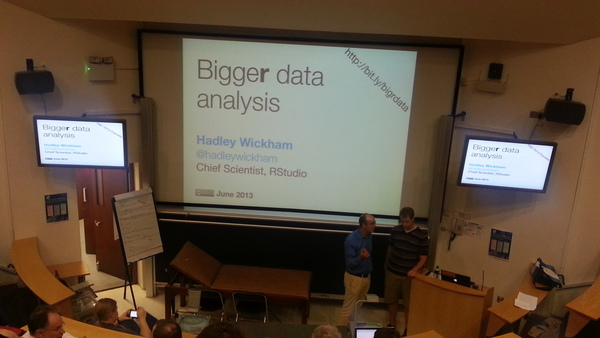
\includegraphics[width=0.99\linewidth]{hadleydublin}

\end{figure}

\end{frame}
%============================================================== %
\begin{frame}
	Prof. Adrian Raftery - Inaugural Gosset Lecture 
\begin{figure}
\centering
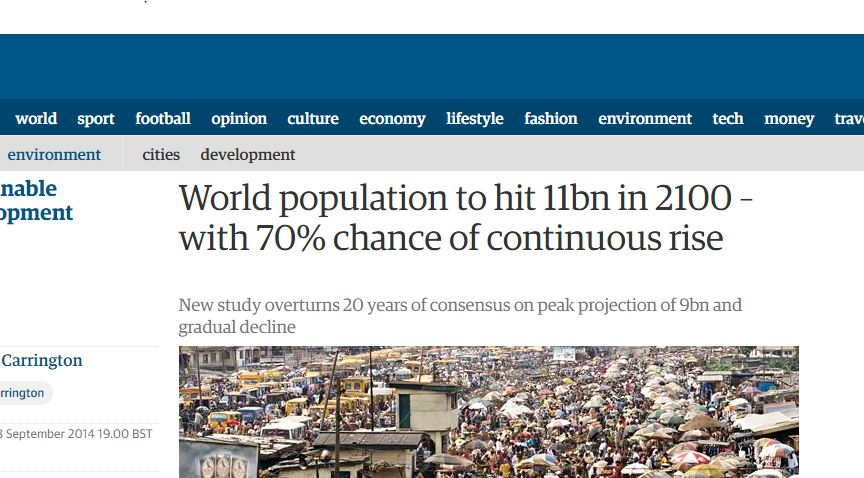
\includegraphics[width=0.99\linewidth]{guardian}
\end{figure}
\end{frame}
\begin{frame}
	Prof. David Speigelhalter at the RIA  -  sell out
	\begin{figure}
		\centering
		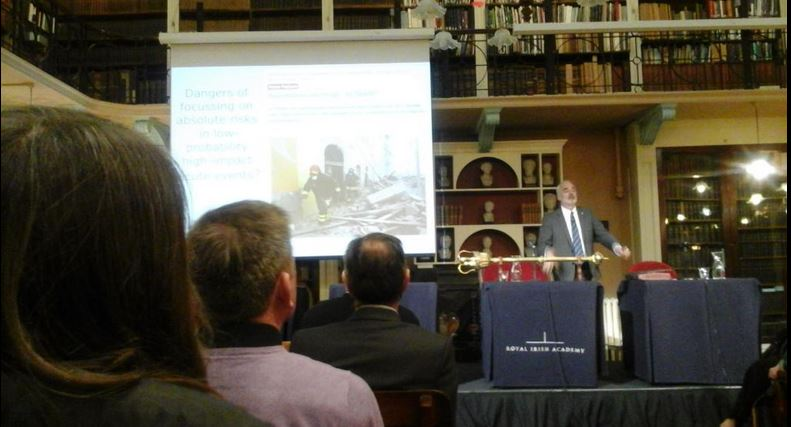
\includegraphics[width=0.99\linewidth]{riaevent}
	\end{figure}
\end{frame}

%=============================================================== %

\begin{frame}
	\frametitle{Diversity}
\Large
\begin{itemize}
\item Tech Bros / Machine Learning Hipsters
\item Coding Grace
\item Beer and Pizza? Worth it?
\end{itemize}
\end{frame}

%================================================================ %
\begin{frame}
	\begin{figure}
		\centering
		
\includegraphics[width=0.99\linewidth]{codinggracelogo}
		
	\end{figure}
	
\end{frame}
%================================================================ %
\begin{frame}
	\begin{figure}
		\centering
		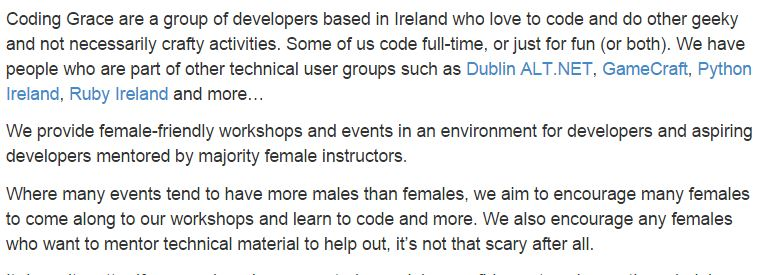
\includegraphics[width=0.99\linewidth]{codinggraceabout}
		
	\end{figure}
	
\end{frame}
%================================================================ %
\begin{frame}
\begin{figure}
\centering
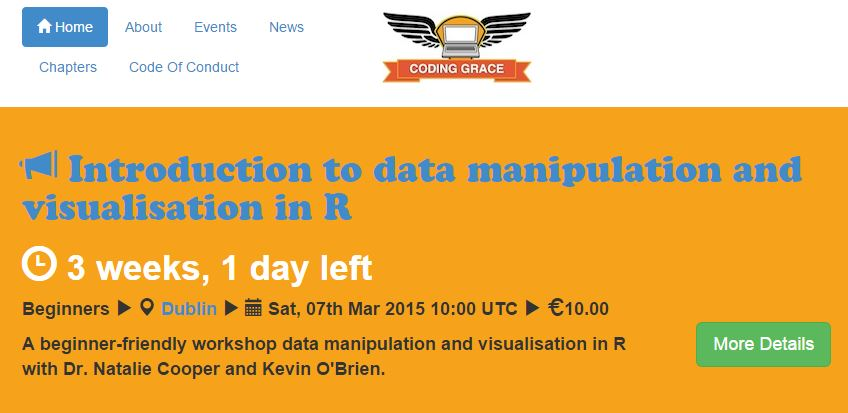
\includegraphics[width=0.99\linewidth]{codinggraceworkshop}

\end{figure}

\end{frame}
%================================================================ %

\begin{frame}
	
	\LARGE
	\textbf{UseR!}
	\begin{itemize}
		\item International R conference
		\item Held every summer
		\item Alternates between Europe and North America
		\item 2015 - Denmark (early July)
	\end{itemize}
\end{frame}
%================================================================ %
\begin{frame}
	\begin{figure}
		\centering
		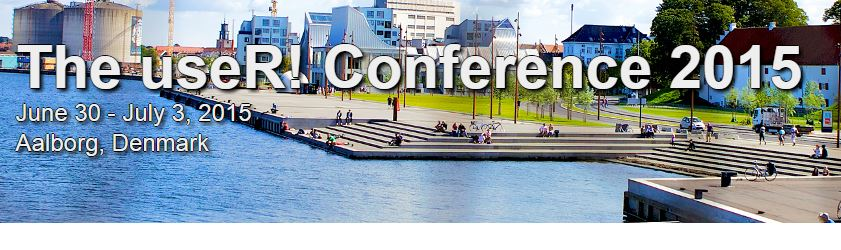
\includegraphics[width=0.99\linewidth]{user1}

	\end{figure}
	
\end{frame}
%================================================================ %
\begin{frame}
	\begin{figure}
		\centering
		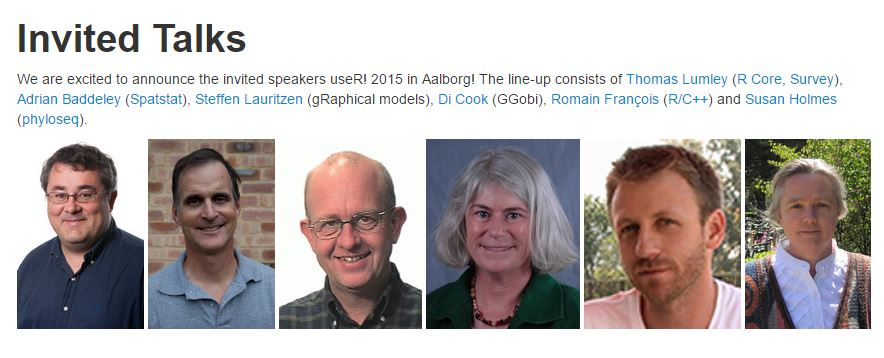
\includegraphics[width=0.99\linewidth]{user2}
		
	\end{figure}
	
\end{frame}
%================================================================ %
\begin{frame}
	\begin{figure}
		\centering
		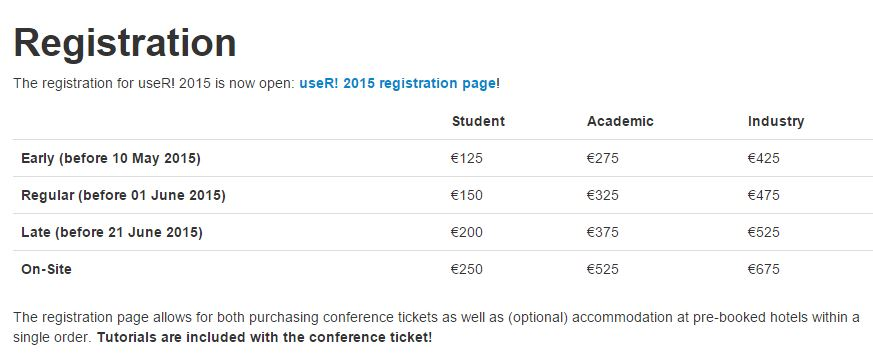
\includegraphics[width=1.11\linewidth]{userprices}

	\end{figure}
	
\end{frame}
%================================================================ %
\begin{frame}
	\begin{figure}
		\centering
		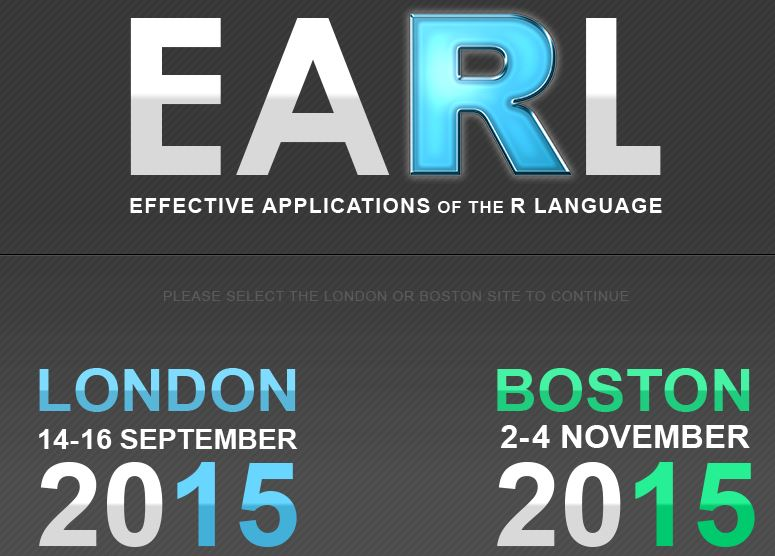
\includegraphics[width=0.88\linewidth]{earlconf1}
		
	\end{figure}
	
\end{frame}
%================================================================ %
\begin{frame}
	\begin{figure}
		\centering
		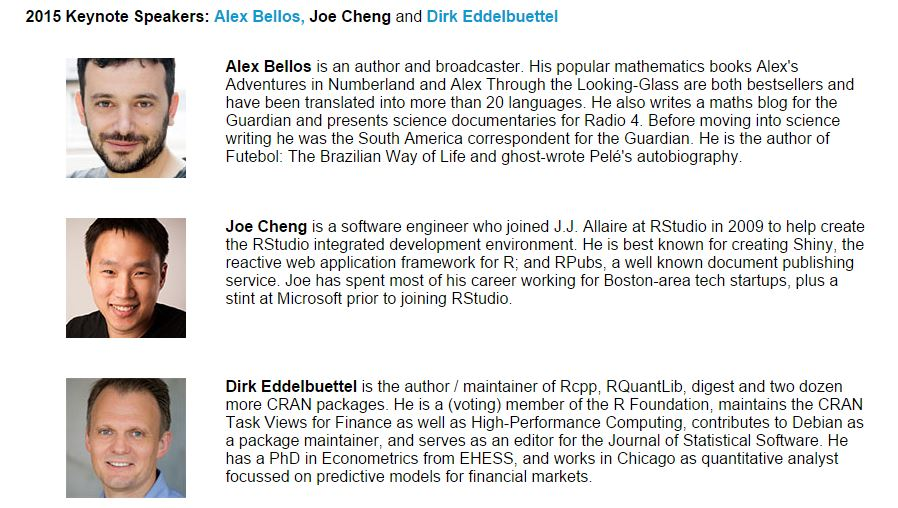
\includegraphics[width=1.11\linewidth]{earlspeakers}
		
	\end{figure}
	
\end{frame}

\begin{frame}
	\begin{figure}
		\centering
		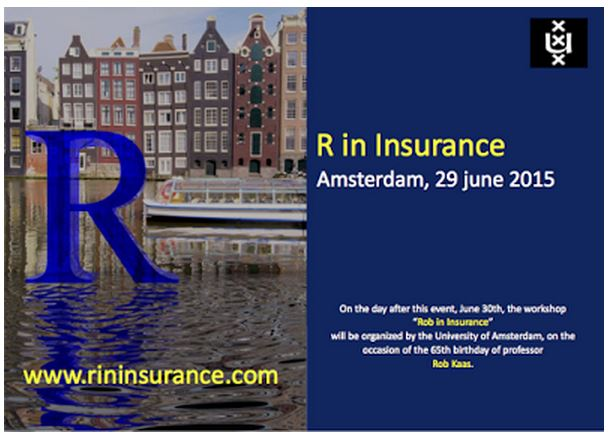
\includegraphics[width=1.11\linewidth]{rininsurance}
		
	\end{figure}
	
\end{frame}
\begin{frame}
	\begin{figure}
		\centering
		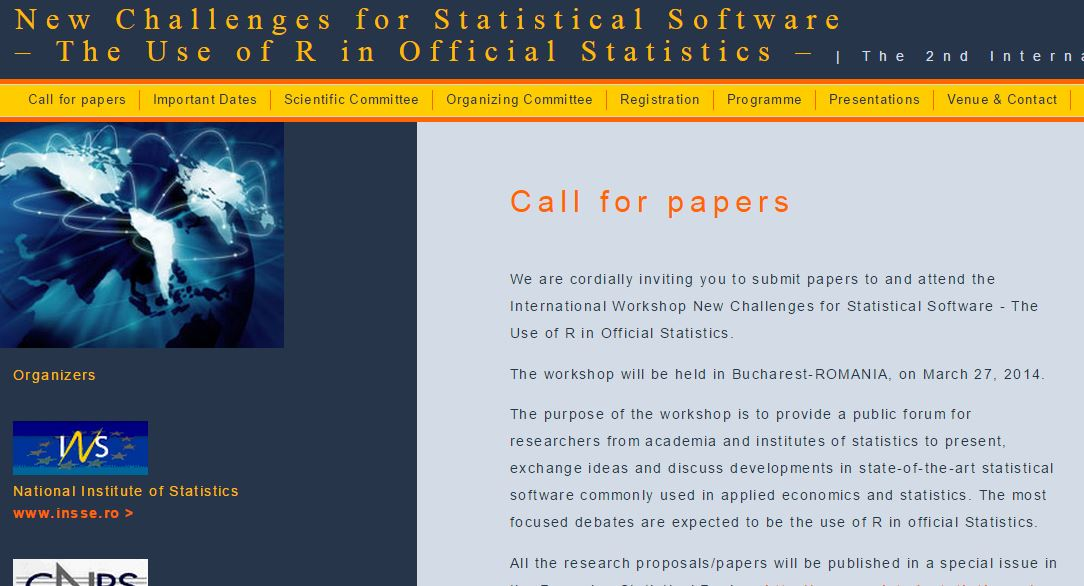
\includegraphics[width=1.11\linewidth]{rofficialstats}
		
	\end{figure}
	
\end{frame}

\begin{frame}
	\begin{figure}
		\centering
		
\includegraphics[width=1.11\linewidth]{sdcmicrocover}
		
	\end{figure}
	
\end{frame}
%================================================================ %
\begin{frame}
\begin{figure}
\centering
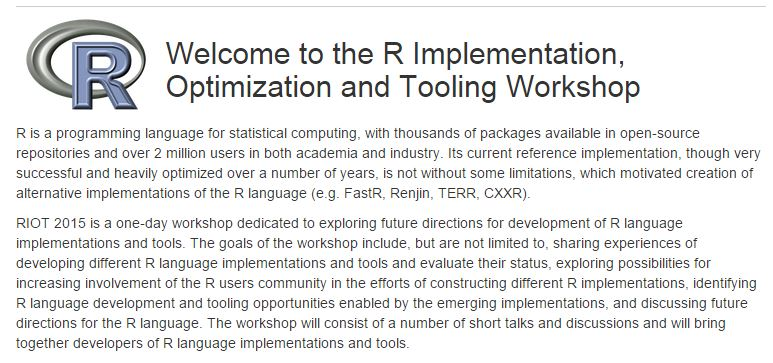
\includegraphics[width=1.11\linewidth]{riot}

\end{figure}

\end{frame}

%================================================================ %
\begin{frame}
	\begin{figure}
		\centering
		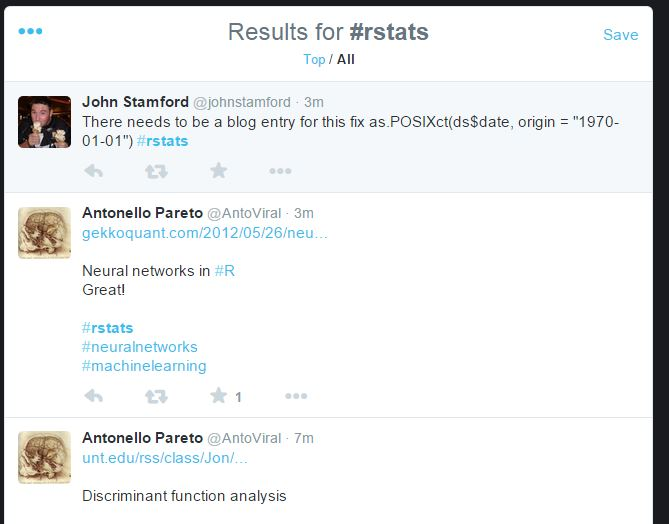
\includegraphics[width=0.88\linewidth]{twitterfeed}
		
	\end{figure}
	
\end{frame}
%================================================================ %
\begin{frame}
	\begin{figure}
		\centering
		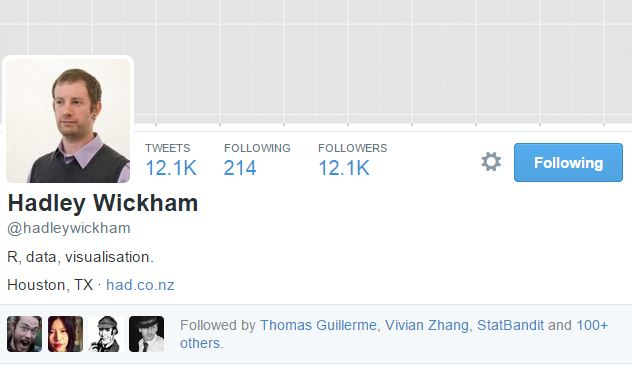
\includegraphics[width=1.1\linewidth]{hadley}
		
	\end{figure}
	
\end{frame}
%================================================================ %
\begin{frame}
	\begin{figure}
		\centering
		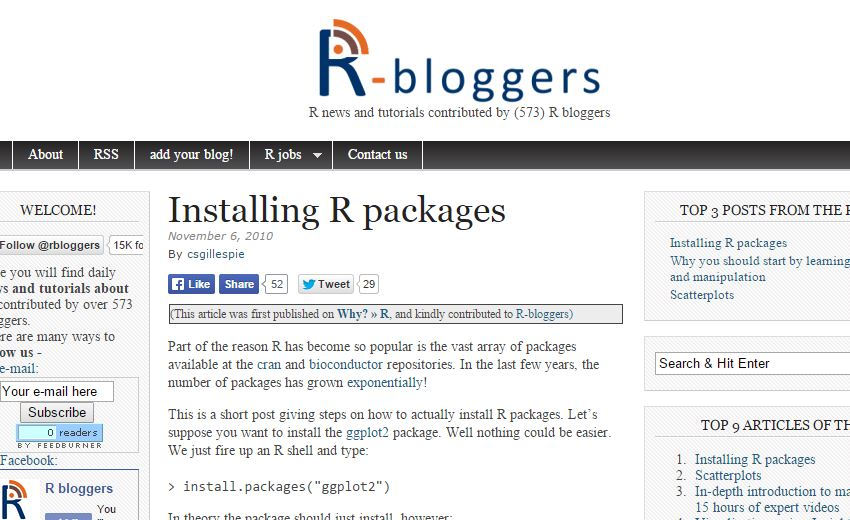
\includegraphics[width=1.05\linewidth]{rbloggers}
		
	\end{figure}
	
\end{frame}
%================================================================ %
\begin{frame}
	\begin{figure}
		\centering
		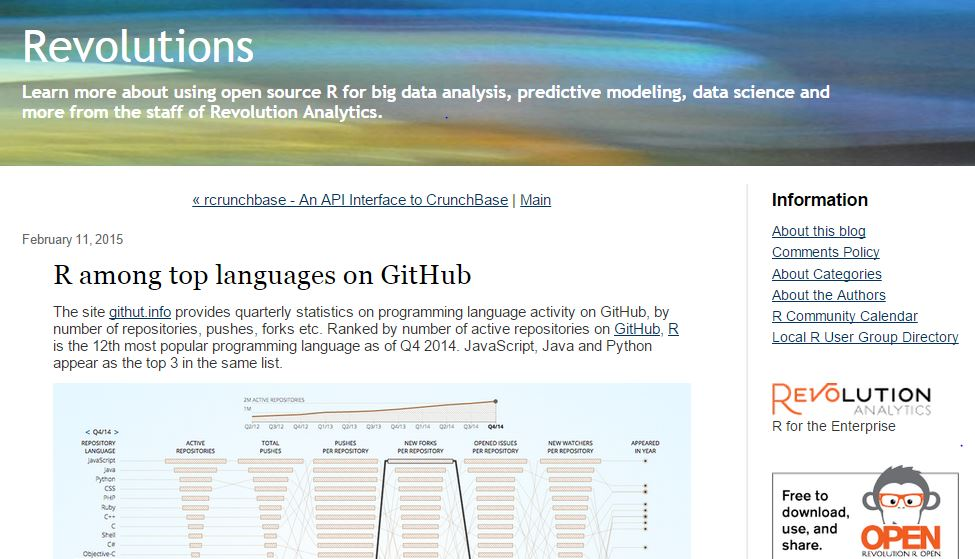
\includegraphics[width=1.05\linewidth]{revoblog}
		
	\end{figure}
	
\end{frame}
%================================================================ %
\begin{frame}
	\begin{figure}
		\centering
		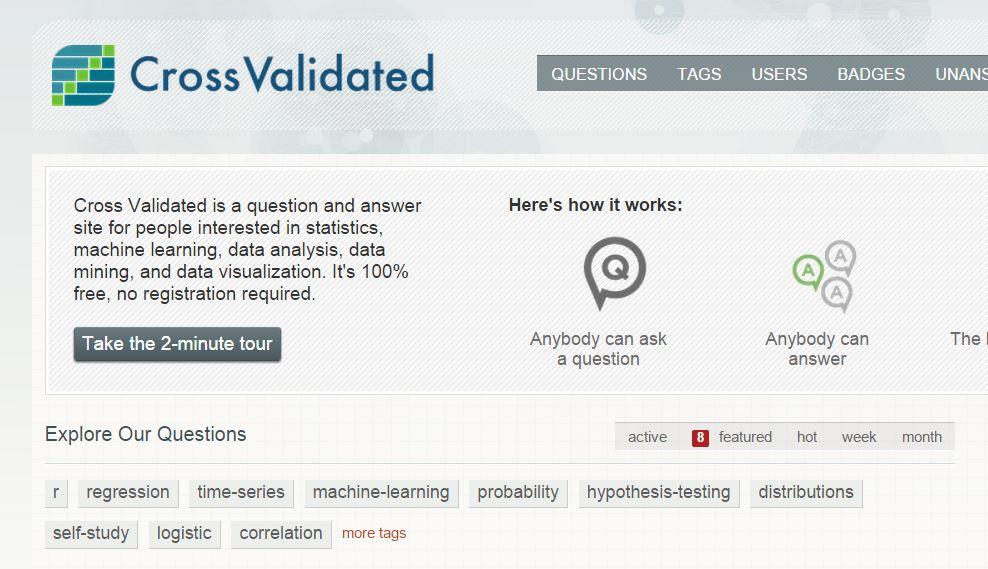
\includegraphics[width=1.05\linewidth]{crossval}
		
	\end{figure}
	
\end{frame}
%================================================================ %
\begin{frame}
	\begin{figure}
		\centering
		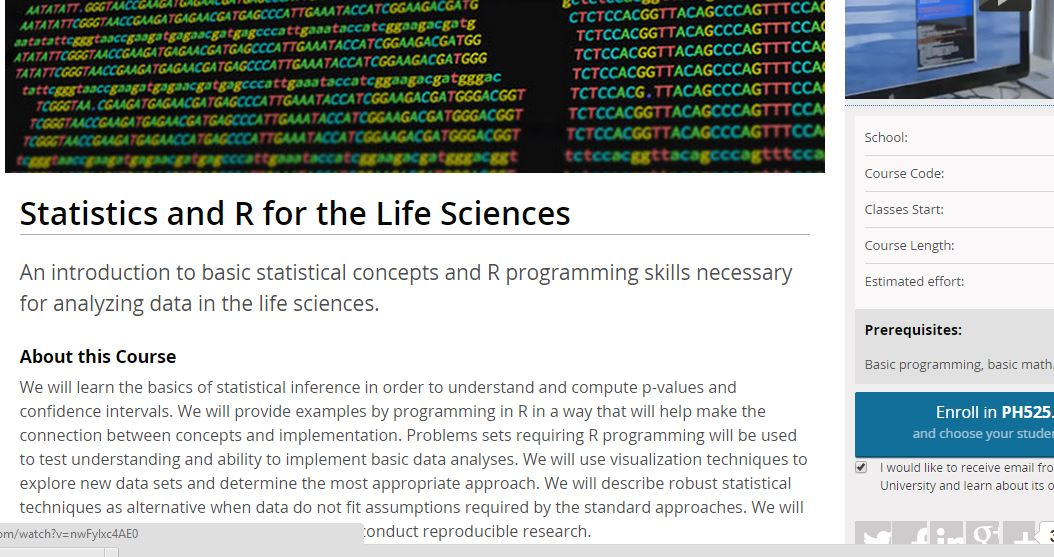
\includegraphics[width=1.11\linewidth]{harvardx}
		
	\end{figure}
	
\end{frame}
%================================================================ %
\begin{frame}
	\begin{figure}
		\centering
		
\includegraphics[width=1.11\linewidth]{courseralogog}
		
	\end{figure}
	
\end{frame}
%================================================================ %
\begin{frame}
	\begin{figure}
		\centering
		
\includegraphics[width=1.11\linewidth]{dss1}
		
	\end{figure}
	
\end{frame}
%================================================================ %
\begin{frame}
	\begin{figure}
		\centering
		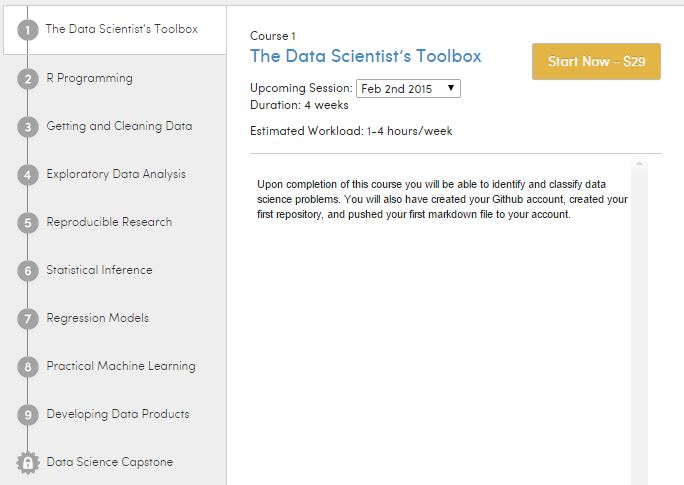
\includegraphics[width=1.11\linewidth]{dss2}
		
	\end{figure}
	
\end{frame}
\end{document}